\documentclass[11pt,a4paper]{article}
\usepackage[utf8]{inputenc}
\usepackage[T1]{fontenc}
\usepackage{tgpagella}
\usepackage[spanish]{babel}
\usepackage{geometry}
\usepackage{graphicx}
\usepackage{booktabs}
\usepackage{array}
\usepackage{xcolor}
\usepackage{titlesec}
\usepackage{fancyhdr}
\usepackage[parfill]{parskip}
\usepackage[expansion=false]{microtype}
\usepackage{hyperref}
\usepackage{setspace}
\usepackage{needspace}

\geometry{top=3.0cm,bottom=3.0cm,left=3.5cm,right=3.5cm}
\setlength{\parskip}{0.65em}
\setlength{\parindent}{0em}

\definecolor{azulai}{RGB}{30,80,140}
\definecolor{doradoai}{RGB}{140,90,0}
\definecolor{grisai}{RGB}{70,70,70}

\titleformat{\section}{\Large\bfseries\color{azulai}}{}{0em}{}[{\color{azulai}\titlerule[0.5pt]\nopagebreak[4]}]
\titlespacing*{\section}{0pt}{1.8em}{0.8em}
\titleformat{\subsection}{\large\bfseries\color{doradoai}}{}{0em}{}[{\nopagebreak[4]}]
\titlespacing*{\subsection}{0pt}{1.4em}{0.5em}
\titleformat{\subsubsection}{\normalsize\bfseries\color{grisai}}{}{0em}{}[{\nopagebreak[4]}]
\titlespacing*{\subsubsection}{0pt}{1.0em}{0.3em}

\pagestyle{fancy}\fancyhf{}
\rhead{\textcolor{grisai}{\small Amaya Ascunce — Arquitectura Interna}}
\lhead{\textcolor{grisai}{\small Carta Natal Completa}}
\cfoot{\textcolor{grisai}{\small\thepage}}
\renewcommand{\headrulewidth}{0.3pt}

\hypersetup{colorlinks=true,linkcolor=azulai,urlcolor=azulai}
\setstretch{1.45}
\tolerance=1500
\emergencystretch=4em

\begin{document}

% ── Portada ──────────────────────────────────────────────────────────────────
\begin{titlepage}
  \centering
  \vspace*{1.5cm}
  {\Huge\bfseries\color{azulai} Carta Natal Completa}\\[0.5cm]
  {\large\color{grisai} Arquitectura Interna}\\[0.3cm]
  {\small\itshape\color{grisai} Un método para sostener cuerpo, energía y vida con coherencia}\\[2cm]
  {\huge\color{doradoai} Amaya Ascunce}\\[1.5cm]
  {\Large 21/02/1979 \quad 17:10}\\[0.3cm]
  {\Large Pamplona, España}\\[0.3cm]
  {\normalsize Lat: 42.8157° \quad Lon: -1.6522° \quad UTC+01:00}\\[0.3cm]
  {\normalsize Ascendente: Leo 15°06' \quad
    MC: Tauro 4°05'}\\[2.5cm]
  \vfill
  {\small Generado el 08/05/2026}
\end{titlepage}

\tableofcontents
\newpage

% ── Rueda ─────────────────────────────────────────────────────────────────────
\section{Carta Natal}
\begin{figure}[h!]
  \centering
  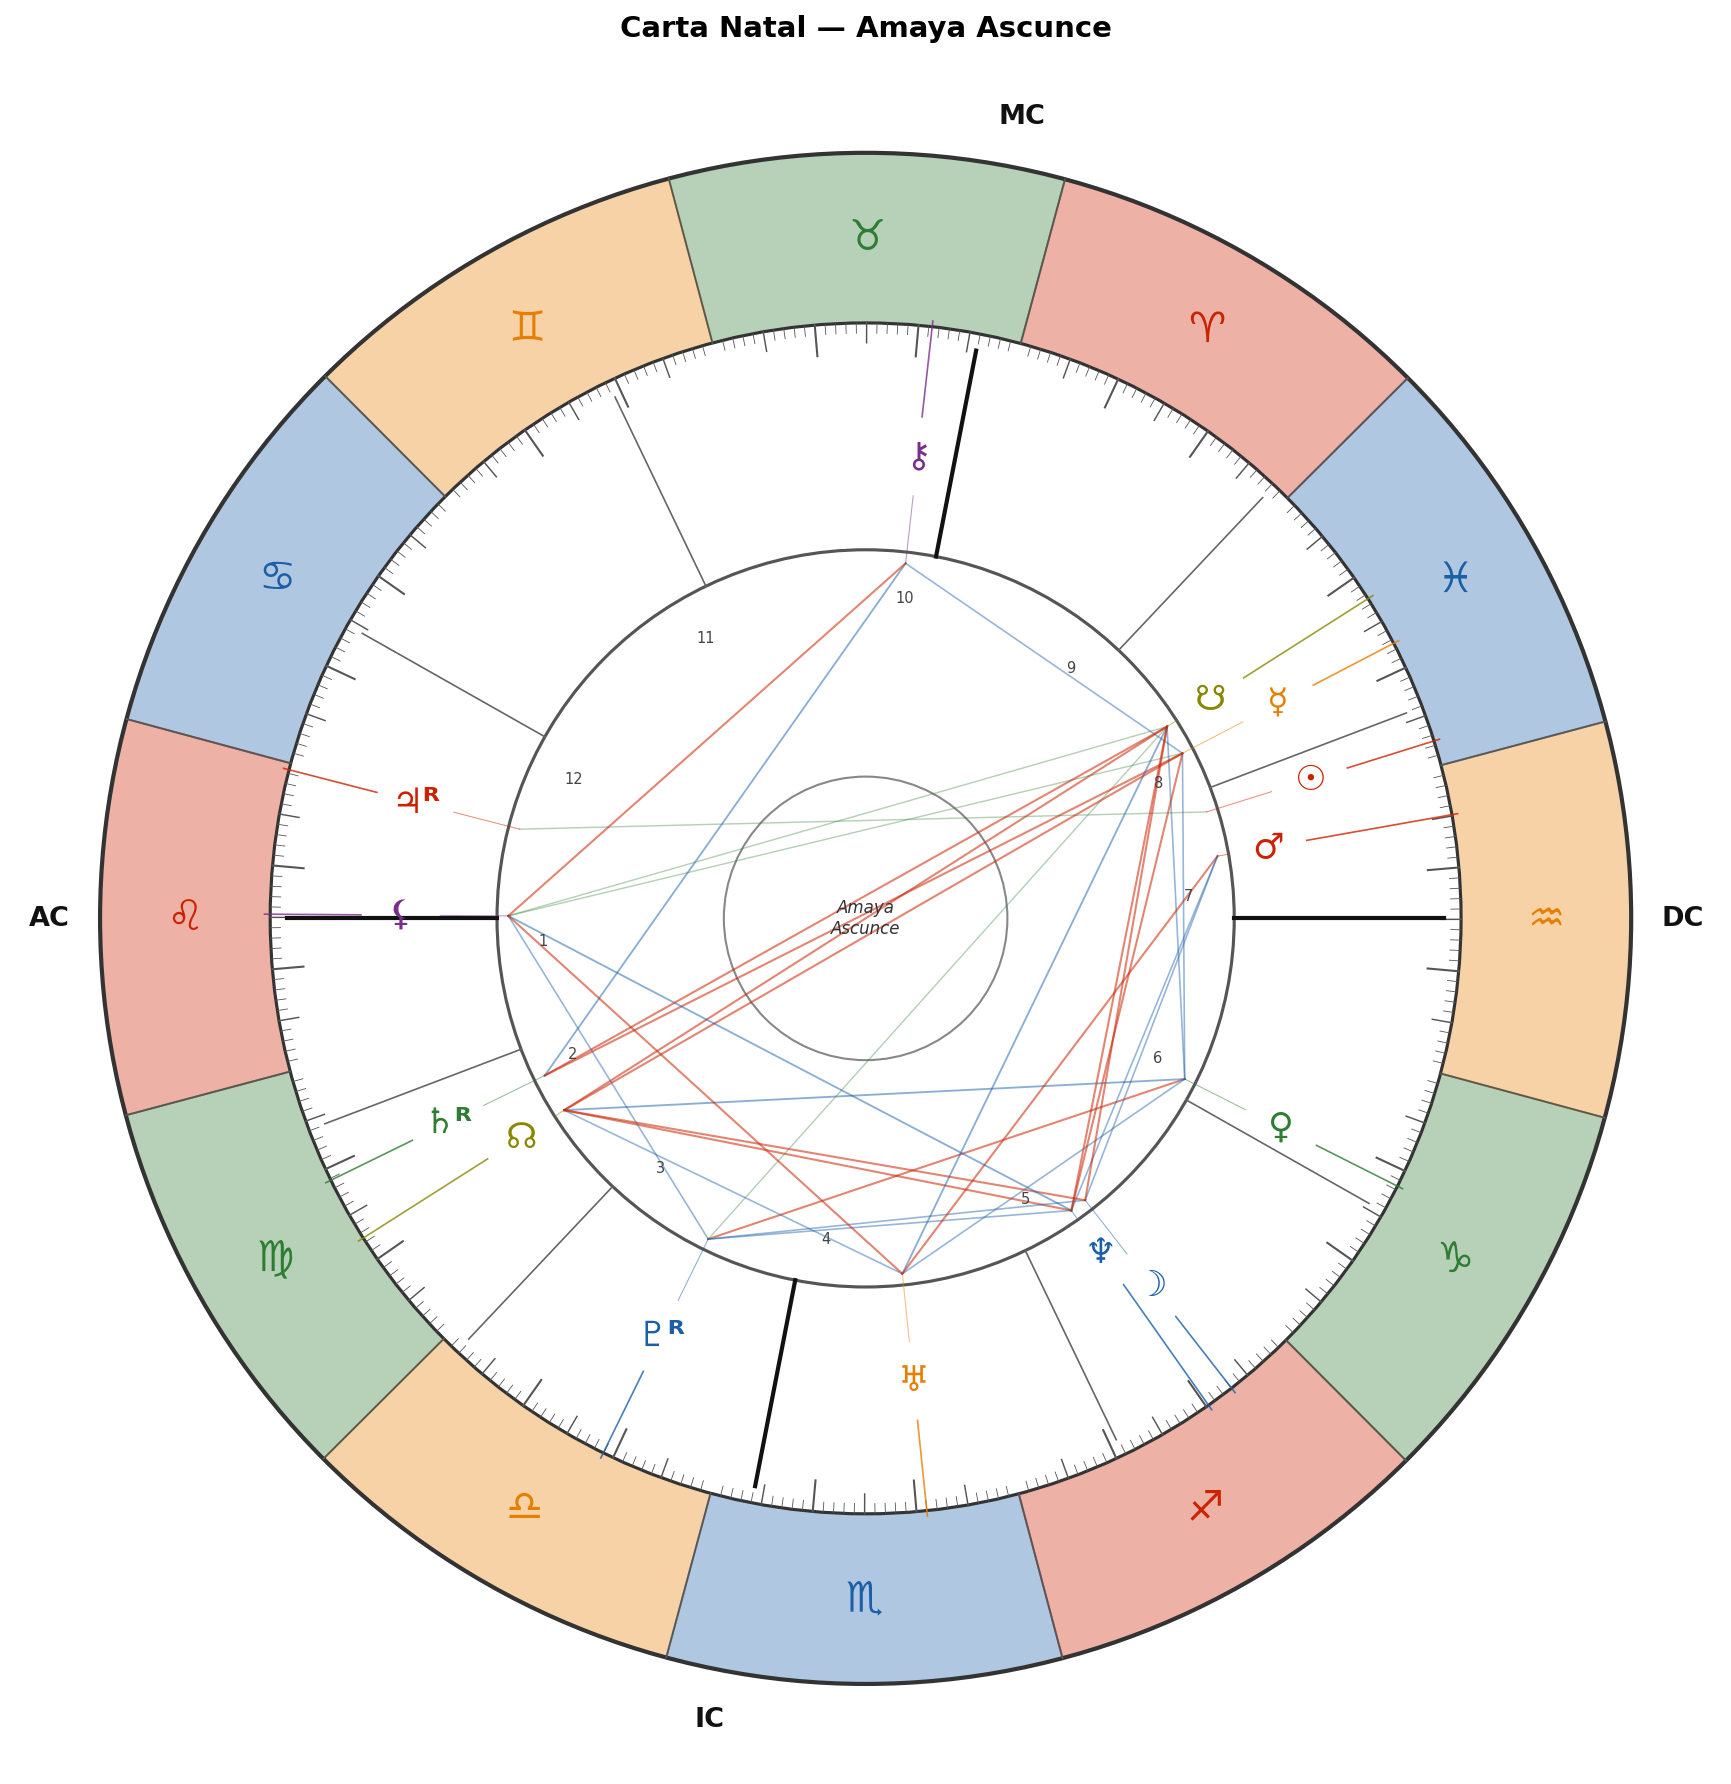
\includegraphics[width=0.90\textwidth]{Amaya_Ascunce_AI_rueda.png}
  \caption{Carta natal de Amaya Ascunce — 21/02/1979 17:10 — Pamplona, España}
\end{figure}

\newpage

% ── Tabla de posiciones ───────────────────────────────────────────────────────
\section{Posiciones Planetarias}

\begin{center}
\begin{tabular}{llrrlll}
  \toprule
  \textbf{Planeta} & \textbf{Signo} & \textbf{Grado} & \textbf{Casa} &
  \textbf{Elemento} & \textbf{R} \\
  \midrule
  Sol & Piscis & 2°26' & 7 & Agua &  \\
  Luna & Sagitario & 23°01' & 5 & Fuego &  \\
  Mercurio & Piscis & 12°37' & 8 & Agua &  \\
  Venus & Capricornio & 18°22' & 6 & Tierra &  \\
  Marte & Acuario & 25°07' & 7 & Aire &  \\
  Júpiter & Leo & 0°38' & 12 & Fuego & R \\
  Saturno & Virgo & 11°11' & 2 & Tierra & R \\
  Urano & Escorpio & 21°00' & 4 & Agua &  \\
  Neptuno & Sagitario & 20°15' & 5 & Fuego &  \\
  Plutón & Libra & 18°57' & 3 & Aire & R \\
  Quirón & Tauro & 8°40' & 10 & Tierra &  \\
  Lilith & Leo & 14°42' & 12 & Fuego &  \\
  Nodo Norte & Virgo & 17°34' & 2 & Tierra &  \\
  Nodo Sur & Piscis & 17°34' & 8 & Agua &  \\
  \bottomrule
\end{tabular}
\end{center}

\vspace{0.5cm}
\begin{itemize}
  \item \textbf{Ascendente:} Leo 15°06'
  \item \textbf{Medio Cielo:} Tauro 4°05'
\end{itemize}

\newpage

% ── Interpretación ────────────────────────────────────────────────────────────
\section{Interpretación — Arquitectura Interna}

\begin{center}
{\small\itshape
No se trata de definirte. Se trata de observar cómo se organiza tu energía,\
dónde puedes perder equilibrio y qué apoyos te ayudan a sostenerte.
}
\end{center}

\vspace{0.5cm}

\subsection{1. Visión General}

Tu carta muestra la siguiente distribución de elementos: Fuego 6, Tierra 2.5, Aire 2.5, Agua 5.5. Fuego (vitalidad, iniciativa, necesidad de sentido y movimiento hacia la acción) y Agua (profundidad emocional, capacidad de resonancia, sensibilidad abierta): ahí está el peso de tu carta. Es el registro desde el que tu energía se activa con más fluidez y sin esfuerzo consciente. La mayoría de tus planetas están en signos mutables: hay facilidad para adaptarte, cambiar y responder a lo que ocurre alrededor. Sueles moverte bien cuando las situaciones evolucionan o requieren flexibilidad. La dificultad aparece cuando todo cambia al mismo tiempo y cuesta mantener una dirección estable durante suficiente tiempo. Tu Medio Cielo en Tauro: La constancia, la paciencia y la construcción de algo sólido con el tiempo. Tu presencia pública suele percibirse como estable y fiable.

\subsection{2. Ejes Principales}

\subsubsection*{Sol en Piscis — Casa 7}
Tu Sol en Piscis funciona con mucha apertura al entorno. Percibes matices, estados y necesidades que no siempre están expresados de forma clara. Eso puede darte sensibilidad y facilidad para conectar con lo que ocurre alrededor, pero también puede hacer que te adaptes demasiado. La dificultad aparece cuando no hay límites suficientes: puedes perder claridad sobre lo que quieres tú. En Casa 7, muchas de las cosas importantes de tu vida se activan a través del vínculo con otras personas. Las relaciones, asociaciones y encuentros significativos suelen tener un impacto directo en cómo te ves. El contacto con el otro te ayuda a reconocer aspectos propios que quizá no verías solo. El riesgo aparece cuando adaptarte al vínculo pesa más que sostener tu propia posición.

\subsubsection*{Luna en Sagitario — Casa 5}
Tu Luna en Sagitario necesita movimiento, perspectiva y sentido. Cuando algo te afecta, te ayuda entender para qué sirve, hacia dónde te lleva o qué puedes hacer con ello. Si no encuentras una salida, el estado emocional puede convertirse en inquietud, impaciencia o necesidad de cambiar de escenario. El movimiento, el cambio de perspectiva y la sensación de amplitud te ayudan a recuperar estabilidad. En Casa 5, tu seguridad emocional se activa a través de la expresión creativa, el juego y el amor. Necesitas que tu vida emocional tenga un componente de disfrute y de expresión auténtica.

\subsubsection*{Ascendente Leo}
Tu Ascendente en Leo hace que te muestres al mundo con calidez, presencia y una orientación natural a ocupar el espacio con seguridad. Entras al entorno con una energía que otros notan. La necesidad de expresarte y ocupar espacio suele percibirse desde el primer contacto. Su regente es Sol, en Piscis y Casa 7. El Ascendente toma el tono de Piscis: sensible, adaptable y muy influida por el entorno. Esa energía opera principalmente desde las relaciones importantes, las asociaciones y el vínculo con la otra persona.


\subsection{3. Organización de la Energía}

Tu Mercurio en Piscis percibe más por imágenes, sensaciones y asociaciones que por lógica lineal. Puedes captar matices sutiles, pero no siempre resulta fácil explicarlos con orden. Te ayuda dar forma poco a poco a lo que percibes antes de intentar comunicarlo. En Casa 8, la mente tiende a profundizar y no quedarse fácilmente en la superficie. Hay interés por entender lo que otros callan, lo complejo o lo que genera intensidad emocional. Tu Venus en Capricornio se vincula con seriedad, compromiso y hechos concretos. El afecto no siempre se expresa de forma expansiva, pero puede ser muy constante. El riesgo aparece cuando protegerte demasiado hace difícil mostrar necesidad o ternura. En Casa 6, el afecto suele expresarse a través del cuidado cotidiano y los gestos prácticos. Estar pendiente de lo que hace falta puede ser una forma importante de mostrar amor. Tu Marte en Acuario actúa de forma independiente y poco convencional. Necesitas sentir que lo que haces tiene sentido propio y no responde solo a una orden externa. El riesgo aparece cuando la resistencia a lo impuesto dificulta colaborar o sostener un ritmo común. En Casa 7, la energía se activa mucho a través de otras personas. Los vínculos importantes pueden generar tanto colaboración intensa como confrontación directa cuando hay tensión.

\subsection{4. Estructura y Tensión}



Los aspectos aparecen organizados en dos niveles. Los aspectos exactos (orbe igual o menor a 1°) suelen sentirse de forma más inmediata y constante en la vida cotidiana. Los aspectos estructurales tienen un orbe más amplio, pero siguen describiendo dinámicas importantes que se repiten a lo largo de la vida.



\Needspace{8\baselineskip}
\subsubsection*{Aspectos exactos}
\Needspace{7\baselineskip}
\subsubsection*{Venus (Casa 6) cuadratura Plutón (Casa 3) --- orbe 0.59\textdegree}
La cuadratura Venus-Plutón intensifica la forma de vincularte. Cuando una relación importa, puede remover miedo a perder, necesidad de asegurar el vínculo o dificultad para soltar el control. No habla de relaciones ligeras: habla de vínculos que tocan capas profundas de deseo, apego y poder personal. Te ayuda reconocer cuándo la intensidad está ocupando más espacio que la relación real.

\Needspace{8\baselineskip}
\subsubsection*{Aspectos estructurales}
\Needspace{7\baselineskip}
\subsubsection*{Plutón (Casa 3) quincuncio Nodo Sur (Casa 8) --- orbe 1.39\textdegree}
El quincuncio Plutón-Nodo Sur señala una tensión entre patrones conocidos y procesos intensos que piden cambio. Puedes permanecer demasiado tiempo en situaciones densas porque, aunque desgasten, resultan familiares. La salida no siempre es romper de golpe; a veces empieza por reconocer cuándo algo ya no transforma, sino que absorbe demasiada energía.

\Needspace{7\baselineskip}
\subsubsection*{Saturno (Casa 2) trígono Quirón (Casa 10) --- orbe 2.51\textdegree}
El trígono Saturno-Quirón indica que la estructura puede ayudarte a sostener zonas sensibles de tu vida. Cuando tienes ritmo, límites y responsabilidades claras, manejas mejor aquello que normalmente te hace sentir inseguridad o exposición. No se trata de endurecerte, sino de crear un contenedor suficientemente estable para no quedar tomado por la vulnerabilidad.

\Needspace{7\baselineskip}
\subsubsection*{Sol (Casa 7) conjunción Marte (Casa 7) --- orbe 7.31\textdegree}
La conjunción Sol-Marte une identidad y acción. Cuando tienes una dirección clara, puedes actuar con rapidez, iniciativa y mucha fuerza disponible. Cuando no hay salida concreta, esa fuerza puede convertirse en impaciencia, tensión o necesidad de intervenir. Este aspecto pide objetivos claros para que la acción no se transforme en desgaste.



\subsection{5. Sostén y Equilibrio}

Tu Quirón en Tauro, Casa 10, señala una zona sensible relacionada con la estabilidad, el valor propio y la relación con lo que necesitas para sostenerte. Puede que hayas vivido inseguridad material o sensación de no merecer descanso, placer o apoyo suficiente. Esto suele notarse especialmente en la vocación, la responsabilidad y el reconocimiento. No significa que tengas límites en ese terreno, pero sí que probablemente necesites más tiempo, cuidado o consciencia para sentir estabilidad ahí.

\vspace{0.3cm}
Tu Nodo Sur en Piscis, Casa 8, muestra una tendencia a moverte desde la falta de límites claros, la adaptación excesiva o la tendencia a perderte en el entorno, especialmente en la intimidad y las situaciones emocionalmente intensas. Suele ser una forma de funcionar conocida o automática para ti. Tu Nodo Norte en Virgo, Casa 2, señala la necesidad de desarrollar desarrollar orden, presencia en lo cotidiano y capacidad de concretar, especialmente en el valor propio y la estabilidad material o emocional. No se trata de rechazar lo anterior, sino de ampliar tu forma habitual de responder.

\vspace{0.3cm}


\subsection{6. Orientación}

\subsubsection*{Qué observar}
Tu Ascendente en Leo describe la forma en que otras personas suelen percibirte al principio. Eso no siempre coincide con cómo vives las cosas internamente o con las tensiones más importantes de tu carta. Cuando hay demasiada distancia entre lo que muestras y lo que realmente te ocurre, aparece desgaste.

\subsubsection*{Qué puede desestabilizar}
Hay ciertas tensiones en tu carta que pueden activarse con bastante fuerza: Nodo Norte-Nodo Sur, Venus-Plutón, Plutón-Nodo Sur. Cuando varias coinciden al mismo tiempo, puede aparecer sensación de saturación, reacción excesiva o dificultad para mantener claridad.

\subsubsection*{Qué estructura y sostiene}
Tu Sol en Piscis, Casa 7, muestra un terreno importante de estabilidad para ti. Cuando tu forma de actuar está alineada con lo que realmente valoras, suele aparecer más claridad y menos dispersión.

\subsubsection*{Orientación práctica}
Una orientación práctica: cuando todo se activa demasiado, no intentes resolverlo todo desde la cabeza. Empieza por algo pequeño y concreto que te devuelva presencia: caminar, ordenar una parte de tu espacio, cocinar, respirar con calma o hacer algo físico y sencillo. Muchas veces el cuerpo recupera claridad antes que la mente.

\vspace{1cm}
\begin{center}
{\small\itshape\color{grisai}
La astrología se usa aquí como lenguaje simbólico de observación, no como una definición de quién eres.\\
Esta interpretación es tu mapa de posibilidades, no tu destino fijo.
}
\end{center}

\end{document}
